% $  Id: validation.tex  $
% !TEX root = main.tex


%%
\section{Validation}
\label{sec:validation}

To validate the appropriateness of CollabIDE, we define two research questions
\begin{enumerate*}[label=(\arabic*)]
\item improve productivity, and
\item SPL
\end{enumerate*} 
To answer these questions, we conducted an empirical evaluation 
to measure how effective CollabIDE was at reducing overhead problems 
in both Distributed Software Development and Software Product Lines.

%%%%
\subsection{Experiment Design}

For each research question, we designed one experiment. In each experiment, we asked 
a group of developers to solve programming tasks using either CollabIDE or a 
conventional IDE following a set of instructions that aim to emulate the workflow that is carried out in each development model. The experiments differ in team sizes, the exercises that need to be solved and the workflow that must be followed to solve the exercises. For the Distributed Software Development experiment, there are groups developers that must each use JavaScript to accomplish their tasks and must also use version control periodically so that both team members code is updated with each other changes. For the Software Product Lines experiment, there are single developers that must use Java or JavaScript depending on the IDE being used to complete their tasks and must also use version control to manage the different product variants that are involved in these tasks. Two metrics are taken in each experiment, first, the percentage of completion of the total tasks assigned and second, the amount of time spent performing actions related to version control.

\authorcomment[missing]{NC}{Context, Research questions, analysis method, data collection method}
CollabIDE está diseñado con el objetivo de reducir el Overhead en los procesos de desarrollo de software en un ambiente distribuido y desarrollo de software con líneas de producción. Con este propósito diseñamos una prueba aislada para validar la efectividad del ambiente de desarrollo en cada uno de estos procesos. En cada prueba se realizó una comparación del desarrollo de una aplicación sencilla en un IDE convencional (i.e., Eclipse o Sublime Text) contra el desarrollo de la misma aplicación utilizando CollabIDE. La descripción de las pruebas y el trabajo de desarrollo se encuentra en el Apendice A.

%%%%
\subsubsection{Experiment 1: Software development in a distributed set-up}
El objetivo de esta primera prueba es cuantificar la reducción de overhead que se logra con CollabIDE en operaciones de envió y obtención de versiones actualizadas de un proyecto que se deben llevar a cabo en un contexto de desarrollo distribuido. 

Para observar dicho objetivo se seleccionaron tres equipos de trabajo, cada uno formado de dos integrantes. Dos de los equipos realizaron el desarrollo utilizando CollabIDE y un equipo de control utilizo Submie Text 3 y git. Cada uno de los equipos tenía la tarea de desarrollar un ejercicio de programación que consistía en implementar operaciones comunes sobre grafos (cf. Apendice A1). La implementación para todos los equipos de trabajo fue realizada en JavaScript. A lo largo de la prueba se tomaron dos métricas, la primera fue qué nivel de completitud alcanzaron los participantes, esto es que porcentaje de los ejercicios lograron implementar en el tiempo límite, la segunda es la cantidad de tiempo que los participantes invirtieron en hacer tareas relacionadas al control de versiones. Para simular el flujo de trabajo en un contexto de ambiente distribuido, los participantes debieron realizar una actualización de sus respectivas versiones cada determinado tiempo, con esta actualización cada participante en un equipo debía quedar con los cambios que el otro miembro de su equipo tenía hasta ese momento. 

%%%%
\subsubsection{Experiment 2: Product variants development and deployment}
El objetivo de la segunda prueba es cuantificar la reducción de overhead que se logra con CollabIDE en operaciones relacionadas al manejo de versiones para crear nuevos variantes en un contexto de desarrollo con líneas de producto. Para observar el objetivo planteado se seleccionaron cuatro participantes. Dos de los participantes realizarón el desarrollo utilizando CollabIDE y los otros dos participantes de control utilizaron Eclipse y git. Cada participante tenía la tarea de desarrollar un ejercicio de programación que consistía en construir 3 variantes de producto a partir de un producto base, en cada variante se tenían que implementar unas determinadas estructuras de datos y unos determinados métodos para cada estructura, las estructuras y métodos a implementar dependían de cada variante (cf. Apendice A2). Los que usaban CollabIDE realizaron la implementación en JavaScript y los otros en Java. Al igual que en la prueba de desarrollo en un ambiente distribuido, se tomaron métricas de nivel de completitud y cantidad de tiempo invertido en control de versiones. Para simular el uso de líneas de producción para el desarrollo de productos se usó el control de versiones en donde una nueva versión del código equivalía a un nuevo variante de producto.  

\begin{figure}[htbp]
  \centering
  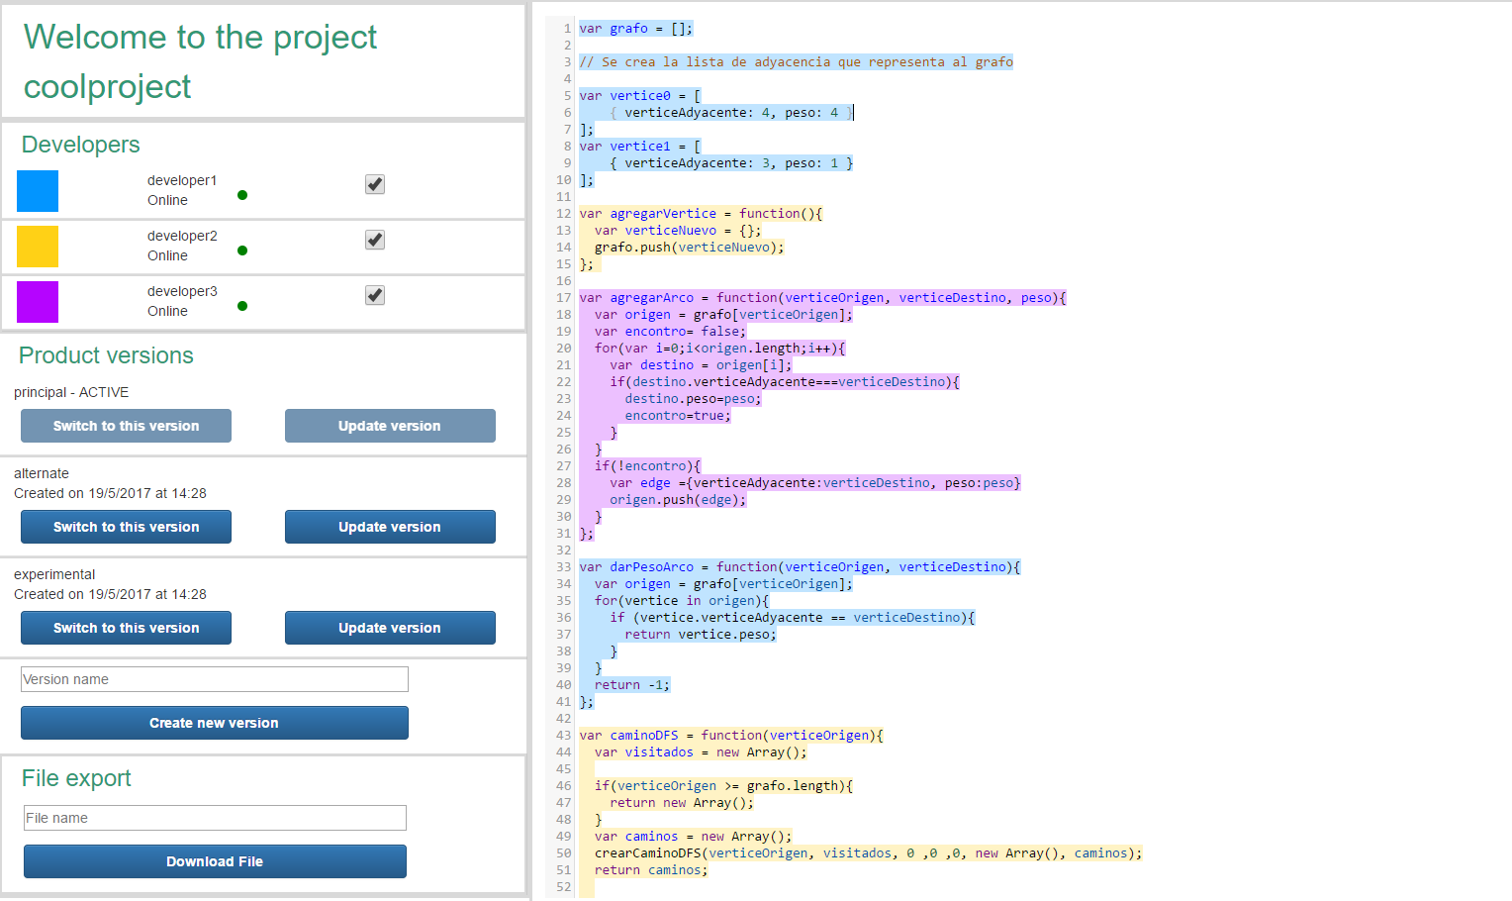
\includegraphics[width=0.7\textwidth]{img/fig1-collabIDEGeneral}
  \caption{CollabIDE tool}
  \label{fig:collabide}
\end{figure}

%%%%
\subsection{Experiment Setup}

Six developers were gathered for the Distributed Software Development experiment, then they were split into groups of two. Two groups would be using CollabIDE and the remaining group would be using Sublime Text in conjunction with git and github. The programming task for this experiment was to implement a set of common graph algorithms using only JavaScript. The participants were given a total of ninety minutes to accomplish this task. Each group was required to obtain their partner’s changes every fifteen minutes using their tools at hand.
In the Software Product Lines experiment, a different group of four developers was gathered. Two of them would be using CollabIDE and the other two would be using Eclipse in conjunction with git and github. In this case, the programming task was to implement a set of data structures with some basic functionality using JavaScript (CollabIDE) or Java (Eclipse). Each data structure also had to be a variant of a given base structure. These participants were also given ninety minutes to complete their task. In order to manage the different product variants, the participants were requested to use version control in each of their IDEs.


\authorcomment[missing]{NC}{Tools, exercise}
	

%%%%
\subsection{Results}

At the end of the experiment, the metrics showed that the developers which used CollabIDE obtained 
a higher completion percentage than those who used the other IDEs. The developers who used 
CollabIDE also spent significantly less time doing actions related to version control than the 
developers that used other IDEs.

%%%%
\subsection{Threads to Validity}
En esta sección discutimos algunos aspectos del experimento que pueden poner en peligro la validez de los resultados. El primero es que la muestra de participantes es muy baja, en el primer experimento tan solo hubo un grupo de control y dos grupos con CollabIDE, del mismo modo en el segundo experimento solo hubo 2 participantes en cada IDE. Cuando las muestras de participantes son bajas, es más fácil caer en el sesgo [11]. El segundo aspecto es que cada experimento duro una hora y treinta minutos, por este motivo se incluyeron pasos específicos en el flujo de trabajo como el de obtener una versión actualizada del proyecto cada 15 minutos, la se hace en intervalos de tiempo más grandes en la vida real. Esta simulación del flujo de trabajo real en ambos experimentos puede también sesgar los resultados en favor de uno de los IDEs.  


\endinput